\chapter{On the origin and evolution of electrical signals\\ during frictional stick slip in sheared granular material}

\section{Abstract}
Electromagnetic signals have been reported in association with geophysical phenomena including earthquakes, landslides, and volcanic events. Mechanisms that suggested to explain seismoelectrical signals include triboelectricity, piezoelectricity, streaming potentials, and the migration
of electron holes, yet the origin of such phenomena remains poorly understood. We present results from laboratory experiments regarding the relationship between electrical and mechanical signals for frictional stick-slip events in sheared soda-lime glass bead layers. The results are interpreted in the context of lattice defect migration and granular force chain mechanics. During stick-slip events, we observe two distinct behaviors delineated by the attainment of a frictional stick-slip steady state. During initial shear loading, layers charge during stick-slip events and the potential of the system rises. After steady state stick-slip behavior is attained, the system begins to discharge. Coseismic signals are characterized by potential drops superimposed on a longer-term trend. We suggest that the observed signal is a convolution of two effects: charging of the forcing blocks and signals associated with the stress state of the material. The long-term charging of the blocks is accomplished by grain boundary movement during the initial establishment of force chain networks. Short-term signals associated with stick-slip events may originate from produced electron holes. Applied to tectonic faults, our results suggest that electrical signals generated during frictional failure may provide a way to monitor stress and the onset of earthquake rupture. Potential changes could produce detectable signals that may forecast the early stages of failure, providing a modest warning of the event.

%% ---------------------------------- %%
%
%  Introduction
%
%% ---------------------------------- %%

\section{Introduction}

A number of electromagnetic signals have been observed during tectonic faulting and mechanical failure of rocks, but the mechanisms underlying these phenomena are still unclear.  Recently, efforts to couple observations by the physics and materials science communities with observations of natural phenomena in the geoscience community have begun to show promise \citep{YujiEnomoto:2007tq,Balk:2009hu,Takeuchi:2010kc,Freund:2010bl,Onuma:2011ii,Shinbrot:2012jd}.  Existing studies indicate that large earthquakes are, in some cases, preceded or accompanied by ultra low frequency electromagnetic emissions, residual magnetic anomalies, and even visible electrical atmospheric discharges known as `earthquake lights' \citep{Derr:1973tq, Park:1993vi, Uyeda:2009du}.  Understanding these phenomena may improve our ability to provide early warning of seismic events or other hazardous material failures, and will provide insight into fault zone physical processes and stress conditions during the seismic cycle.  

Several mechanisms have been proposed to explain the generation of electrical potentials in Earth, including: piezoelectric effects, streaming potential, contact/tribo electrification, fracto-emission, plasma excitation, and semiconductor-like effects \citep{Finkelstein:1973vz,Dickinson:1982hx,Dickinson:1982uy,Dickinson:1984ft,Freund:2000vf, Frid:2000vn, Jouniaux:2013da,Takeuchi:2013cu}.  Even with an assumed mechanism of charging, there are still many mysterious aspects of the phenomenon, including conduction of the charge to the surface, charge residence time, and Earth/atmosphere interaction. Here, we examine electrical potentials observed for sheared granular layers that exhibit regular frictional stick-slip instabilities in the laboratory.  We interpret the results of experiments on this fault gouge analog in the context of modern theories of charge separation in geologic materials. 

%% ---------------------------------- %%
%
%  Previous Work
%
%% ---------------------------------- %%

\section{Previous Work}

\subsection{Natural Occurrences}
Light emissions have been reported in association with rock failure during both seismic rupture at Earth's surface (so-called Earthquake lights) and during rock bursts in mines.  Earthquake lights have been reported during various stages of the seismic cycle, in addition to other electromagnetic phenomena.  Related electrical phenomena believed to be connected with rock failure include ultra low frequency electromagnetic emissions, resistivity variations \citep{Park:1993vi}, and anomalous animal behavior \citep{Kirschvink:2000wu}.  A summary of these phenomena by\citet{Uyeda:2009du} and the references therein illustrate the breadth of observations.

The first photographically well-documented sequence of earthquake lights (EQL) occurred during the 1965-1967 Matsushiro earthquake swarm \citep{Derr:1973tq}.  Earthquake lights were also observed in the M7.2 November 29, 1975 Kalapana earthquake.  The M7.2 1995 Kobe earthquake was reported to have EQL as well as observations of burned plant roots at the rupture site, and natural remanent magnetization (NRM) anomalies \citep{YujiEnomoto:2007tq}.  Anomalous NRM have been measured in pseudotachylyte, suggesting that high remanent magnetizations were acquired in a co-seismic electrical process and locked into thin, rapidly cooling layers of melt \citep{Ferre:2005ci}.  Visual electromagnetic phenomena were reported before the M6.3 April 6, 2009 L' Aquila earthquake \citep{Fidani:2010ie}. Although reports were confused by astronomical/meteorological events and coseismic power line flashes, a number of unexplained observations remain.

Most reported EQL have been generated on intraplate faults with relatively shallow sources, for magnitude 7 and greater events, and commonly for earthquakes with demonstrated surface rupture.  \citet{Lockner:1983ux} suggest that vaporization of water produces a charge separation that is then moved to the surface by a central fluid conductor.  Reports of EQL phenomena often include descriptions of the anomalies being most intense at topographic highs, suggesting that surface charge on the ground was concentrated by the topography. EQL may be more common in high stress drop events and/or in association with branching and geometrically complex events \citep{scholz2002mechanics}.

\subsection{Previous Experimental Work}

Much experimental work has been done to test physical mechanisms that could cause electrical anomalies during seismic activity and rock failure.  The most relevant explanations are briefly discussed here, but more in depth discussion may be found in \citet{Uyeda:2009du}, \cite{Freund:2000vf}, and references therein.

Early work by \citet{Nitsan:1977te} investigating piezoelectric effects showed electromagnetic radiation in the 1-10 MHz range during the fracturing of quartz bearing rocks under uniaxial compression.  The idea of the piezoelectric effect causing changes in the electrical field during failure suggested that frequency content of the signal would be related to the rate of stress release.  This relationship is supported by a spectral shift to higher frequencies with smaller particles \citep{Nitsan:1977te}.  Uniaxial compression studies using cores of Red Texas Granite, Barre Granite, Dakota Sandstone, Carthage Marble, and quartzite exhibited electromagnetic signals peaking below 40 kHz in association with failure. Observed signals also exhibited some degree of directionality \citep{Rowell:1981tp,Hanson:1982vu}.  Signals peaking at 100 kHz were observed during impact and cratering tests by \citet{Bianchi:1984vf} both in vacuum and at atmospheric pressure.

Mechanisms involving the formation of cold plasmas during fracture and impact have also been proposed to explain charge generation \citep{Martelli:1985wv}, but have not been investigated thoroughly.  Calculations considering a beam-plasma interaction producing an ion-acoustic instability suggest that the expected radiation frequencies are at $\sim$50 kHz.  

A recent study by \citet{Onuma:2011ii} examined gabbro and quartz powders, used as simulated fault gouge and sheared between gabbro forcing blocks in a saw-cut geometry.  Electrical signals in the co-seismic period were detected by direct contact electrodes as well as toroidal induction coils surrounding the sample.  In 25\% of their experiments, a possible pre-cursory signal was detected, but not consistently on all instruments.  Piezoelectricity was ruled out as a dominant mechanism, because signals were observed in piezoelectric and non-piezoelectric gouges and there was no preferred c-axis orientation in the quartz powder.  Signals were observed from piezoelectric and non-piezoelectric materials by \citet{Cress:1987wy} as well, but in their experiments on quartz produced larger signals than other materials.  \citet{Onuma:2011ii} did not observe signals during initial loading; however, such signals have been observed by other workers in natural and experimental cases \citep{Takeuchi:2010kc} who attributed them to frictional electrification because they scaled roughly linearly with slip.

The presence of moving dislocations with respect to propagation of microcracks producing a `pressure stimulated current'  in marble samples has been examined \citep{Triantis:2008uo}.  These currents are a result of charge separation during the beginning stages of failure, not during the initial loading stages.  

Piezoelectric effects are well-documented in materials such as quartz, but geologic materials are not expected to have the required mineralogy or grain alignment to make this a viable mechanism in nature.  Randomly oriented grains would produce a series of randomly oriented dipoles that would cancel to produce a net-neutral field.  Streaming potentials and electrokinetic effects \citep{Mizutani:1976tn} are well-documented, but are generally not of sufficient magnitude to explain the observed phenomena, because large potentials are difficult to maintain with generally conductive fluids present.  Electrification by relative surface movement (tribo-electrification) is also well-documented \citep{Pingali:2009je,Pahtz:2010cq}, but does little to explain electrical signals produced while contacts are stationary to quasi-stationary. 

Evidence for electrical signals during and possibly as precursors to failure in a low stress environment has been collected \citep{Shinbrot:2012jd} in experiments examining slope failure and crack opening or closing in powdered pharmaceutical materials.  An electrostatic voltmeter (ESVM) like that used in this study was used to monitor rotating and tilting drums of powder as well as flexure of powder layers resulting in opening and closing fissures of the material. 

Another model of charge generation during deformation of geomaterials is the `semiconductor' effect.  In geologic materials, oxygen is generally considered to exist in the O$^{-2}$ valence state, but the more oxidized form O$^-$ is also present in a pair of coupled O$^-$ atoms known as a peroxy defect.  The peroxy link can be broken via mechanical strain such as during passage of a mechanical deformation front in the form of a propagating elastic wave or elastodynamic rupture front. In this case, an electron is sourced in an attempt to satisfy the newly formed electrical imbalance at the site of the broken peroxy bond.  This oxidizes the donor, forming a single defect electron (eq.\ref{peroxy}). \citep{Freund:2000vf, Freund:2006kb,Freund:2010bl}
  
\begin{equation}
O_3 X/^{OO}\backslash YO_3 + [XO_4]^{n-} \leftrightarrow O_3X/^{O} \bullet _O/YO_3+[XO_4]^{(n-1)-}
\label{peroxy}
\end{equation}

Electrons are not free as charge carriers, but holes remain mobile \citep{Freund:2000vf,Freund:2006kb,Freund:2010bl,Balk:2009hu}. The semi-conductor effect has been explored in solids \citep{Takeuchi:2013cu,StLaurent:2006fq}, but few studies have been conducted on granular materials, which are likely to be important in the behavior of tectonic fault zones.

%% ---------------------------------- %%
%
%  Methods
%
%% ---------------------------------- %%
\section{Methods}

We conducted experiments on granular layers used to simulate fault gouge under controlled boundary conditions, with concurrent measurement of electrical potential, stresses, and strains of the layer to explore the relationship between stress state and the evolution of electrical signals.  We used glass beads to represent granular fault gouge because they exhibit repeated frictional stick-slip behavior and share key friction constitutive properties with rock. The main advantage of this choice lies in the reproducibility of stick-slip behavior, allowing investigation and isolation of the processes that cause electrical signals relevant to natural faults containing granular gouge by using a simple, well-characterized system. We note that glass should contain fewer starting defects than silicate minerals found in natural fault gouges, such that any effects observed in our glass bead experiments would likely be amplified in natural materials.

\subsection{Apparatus}

All experiments were conducted on a biaxial deformation machine with a servo-hydraulic control system \citep{Karner:2000tj,Frye:2002jj}.  Hydraulic servo valves are operated in either displacement or force feedback modes through a series of analog amplifiers and comparators.  Control displacement signals are generated by a 16-bit digital to analog converter capable of $\pm 5$V range.  The apparatus (Figure \ref{biax_setup}A) is capable of 1 MN of force on the horizontal ram and 1.5 MN on the vertical ram.  Ram velocity can be controlled to ~0.1 $\mu m/s$ in displacement mode, or to about 10N in load mode \citep{Hong:2005gd,Rathbun:2008ks}.

We used forcing blocks of cast acrylic with a dielectric strength of 15-17 V/$\mu m$ and a tensile strength of 55-77 MPa.  Forcing blocks were cut to size and machined with grooves 1 mm deep and 2 mm wide perpendicular to the shearing direction to ensure that shear occurred within the layer and not at the layer boundary \citep{Anthony:2005jo,Knuth:2007ci}.  Acrylic side shields were also made to confine the sample material. The nominal frictional contact area was 10 cm x 10 cm.

Force was measured using Beryllium-Copper strain gauge load cells built in-house and placed in series with the loading ram and sample. The load cells and the wheatstone bridge electronics are calibrated regularly with a proving ring traceable to the National Bureau of Standards.  Displacement is measured with direct current displacement transducers (DCDTs) affixed to the ram nose and referenced to the end platens of the hydraulic rams.  Positions of both classes of instrumentation are noted in Figure \ref{biax_setup}A. 

We recorded data using a 24-bit, 16-channel simultaneous, delta-sigma style analog to digital system.  Samples are collected at 10 kHz and averaged to the desired rate from 1 Hz to 10 kHz as necessary to maintain the appropriate signal-to-noise ratio.  Recording rates may be changed during the experiment, and our tests show minimal cross-talk or dwell errors in this system.

\subsection{Sample Material \& Preparation}
Samples were built in the double direct shear configuration (Figure \ref{biax_setup}B) using soda-lime glass beads \citep{Anthony:2005jo}.  Two layers of beads were confined in a three forcing block assembly with a rubber membrane at the bottom and side-shields on the boundaries to avoid lateral extrusion of the material.  The top of the sample was unconfined. 

Layers were built by placing the side forcing blocks on a leveling jig and applying cellophane tape around the perimeter.  The tape was then trimmed to the desired height to produce uniform, reproducible layers. We used 5 mm thick layers for all experiments in this study (Table 1).  Sample material was poured into the form, lightly compacted, and leveled.  The center forcing block was affixed to one side block (and the sample) with additional cellophane tape, securing the blocks and gouge layer and providing enough strength to allow transport of the sample from the bench to the deformation apparatus. The process is repeated for the second layer.

We constructed layers using Class IV soda lime glass spheres (product GL0191B4/106-150) from Mo-Sci Specialty Products in Rolla, Missouri (composition shown in Table \ref{bead_composition}).  Two mono-disperse size distributions were tested: 100-150 $\mu m$ and 420-500 $\mu m$. Scanning electron microscopy (SEM) analysis of the beads shows that they are homogeneous, with few exceptions, and smooth (Figure \ref{starting_SEM}). Past work has shown that bead comminution is minimal until $\sigma_n>10$ MPa \citep{Mair:2002hu,Mair:2011fd}.  

\subsection{Potential Measurement}
Electrical potential on the layers was measured by a model 344 electrostatic non-contact volt meter (ESVM) manufactured by Trek Inc.  This instrument reported the potential with respect to system ground sensed in its field of view. An analog output of the measured voltage was divided by 100 to provide a sensing range of $\pm 2$ kV with a $\pm 20$ VDC output signal recorded.  A `response' setting on the instrument controlled internal damping constants.

The sensor head contains two electromechanically oscillated plates.  Plates are fixed parallel to each other with the surface normal facing the surface under test.  The front plate is affixed to the instrument body and has a small aperture in the center. The rear plate is inside the instrument and is the oscillating plate.  The sensor operates by varying the voltage across the plates and sensing the alternating current (AC) signal resulting from the movement of the plates with respect to one another.  When the AC component of the signal is nulled, the voltage across the plates exactly matches the voltage on the surface under test.  This sensor configuration has several advantages: 1) no contact is required with the surface under test, which is excellent for systems where coupling is a challenge, 2) there is no arcing risk since the instrument and surface under test are at the same potential, and 3) the sensor is easily portable, allowing tests with different viewing positions.

Two different sensor geometries were used: side view and top view (Figure \ref{biax_setup}C).  In the top view, all tape between the sensor and the sample was removed.  In the side view, a notch was cut in the side shield, leaving only a thin layer of tape (necessary to prevent extrusion) for the sensor to observe through.  In our calibrations, we found that the sensor operates normally when viewing signals through thin obstacles.  

\subsection{Experimental Procedure}
Samples were placed into the testing machine and normal load of 4 MPa was applied and maintained to compact the layers.  The shear load was then applied by driving the vertical ram at a constant displacement rate (1, 30, or 100 $\mu m/s$).  Electrical potential was recorded by placing the sensor in either the top or side view geometry with a distance of $\sim$1 cm between the front of the sensor and the gouge layer.  The response setting was set to the maximum value of 9.  
	 
We conducted experiments at room (ambient) humidity, at 100\% relative humidity (RH), and under submerged conditions using de-aired water.  100\% RH was achieved by placing the sample assembly in a plastic membrane with a beaker of anhydrous sodium carbonate solution (2:1 ratio with distilled water) within the membrane.  This exothermic reaction produced a 100\% RH environment in the membrane.  For all experiments under controlled humidity, samples were left to equilibrate overnight with a small normal stress applied by a hand-clamp, and then placed in the testing machine. When the experiment began, we refreshed the anhydrous sodium carbonate solution, applied the normal stress and proceeded with our standard loading protocol.  For these experiments, we cut a small window in the humidity-control membrane to provide access for the sensor.  A capacitive sensor hygrometer (Lifft C200 with a maximum error of $\pm3\%$) verified that the relative humidity never fell below 100\%.  Saturated experiments were performed in a similar manner, but the membrane was filled with distilled water and the sample allowed to saturate as load was applied.  The water level just covered the top of the blocks and a top-view ESVM geometry was employed. 

\subsection{Calibration and Control Tests}
We performed tests to ensure calibration of the ESVM, as well as to evaluate the sensitivity of the response control.  The ESVM probe was affixed to an electrically insulating base and placed approximately 1 cm from an aluminum plate.  The plate was charged with a precision DC power supply (HP 6216B) and the true and measured plate voltages recorded. Performance was further evaluated by attaching the surface under test to a function generator.  Square waves were measured on each response setting (1-9) to evaluate ringing of the instrument (Appendix A).

In addition, an experiment identical to those testing electrical potential on the layers was performed with the ESVM pointed away from the load frames into the room and towards a DC charged aluminum plate.  This test was performed to ensure that the signals we observed during shearing were not from electrical interference of the hydraulic control electronics or measurement/recording electronics.  We note that our records include motion of the vertical hydraulic ram when it was not in contact with the sample, and no change in voltage was seen.  This further indicates that no DC offsets or interference were experienced by the ESVM from the testing machine and/or control electronics and transducers.


All calibration and control tests were conducted with identical analog to digital conversion hardware as the experiments.  ESVM calibration tests were also conducted on an independent logger (the LabJack U6) to ensure there was consistent performance and minimal measurement burden from either system.


\subsection{Data Analysis}

Changes in electrical voltage during stick-slip events were picked by hand to evaluate the electrical signal.  ESVM data are more noisy than the mechanical data and electrical anomalies are not found with every stick-slip event, making manual picking the most accurate.  Measured electrical potential and shear stress were plotted on the same x-axis and mouse position clicks were recorded.  Interpretation was aided by superposition of a smoothed potential signal.  The potential was smoothed using a Savitzky Golay filter \citep{SG1964}, as it preserves peaks, but decreases noise.  With the Savitzky Golay filter, a line of specified low-order is fit to a certain data window using a linear least squares technique.  The analysis is then stepped forward and fit signals convolved.

 Data were recorded in a binary form, decoded, converted from bits to engineering units through use of calibrations derived from our transfer standards, and then written out as either a binary or ASCII for analysis. The Python environment was used for processing and analysis.  All stick-slip events were automatically picked by first computing the smoothed derivative of shear stress with respect to time using a running-average slope tool.  Zero-crossings of the derivative indicate a slope change from positive (like that during load up) to negative (like that during failure) or the reverse.  The automatically determined stress drops were checked against a threshold value to ensure that no noise was picked as events.  Automatic picks were visually inspected to ensure algorithm performance.  

\section{Results}

\subsection{Mechanical Data}
The application of shear load resulted in a characteristic linear-elastic stress-displacement record during initial run-in (Figure \ref{ss_humidity}).  Stick-slip behavior began as we reached the failure strength of the material.  As shear load increased during the stick-slip cycle, the material began to creep and deform elasto-plastically, as indicated by deviation of the stress-strain curve from the initial, linear-elastic trend.  When the ultimate strength of the layer was reached, layers failed and a stress drop was observed.  We define the stress drop as the magnitude of shear stress change during stick-slip failure.  In a series of repeating events, we define the recurrence time as the time between peak stresses of two slip events.  For a summary of this terminology see Figure \ref{ss_humidity} inset.  Mechanical steady-state (not to be confused with steady-state frictional sliding) refers to the system state after the initial run-in period, defined as the point at which stress drops in repeated stick-slip events become constant.

All experiments exhibited a maximum coefficient of friction during mechanical steady-state ($\mu \equiv \tau / \sigma_n$) of 0.3-0.4.  For experiments at 100\% humidity or water saturated, we observed an increased stress drop and ultimate strength due to the activation of chemo-mechanical mechanisms such as solution-reprecipitation \citep{Frye:2002jj, Yasuhara:2005ku, Scuderi:2013}.

The recurrence time between events has been shown to vary with load point velocity \citep{Karner:2000tj,Beeler:2001tj}.  We observe a power law relation between load point velocity and recurrence time with a characteristic slope of -1.14 (Figure \ref{ss_props}A).  For faster load point velocities, there is less time for contact healing to occur before the layer fails, resulting in lower maximum stresses and shorter recurrence times.  Shorter healing times also result in smaller stress drops, which produce a correlation between longer recurrence times and larger stress drops (Figure \ref{ss_props}B).  

Experiments performed using the 420-500 $\mu m$ glass beads exhibited repeated stick-slip behavior and a lower coefficient of friction of $\sim 0.2-0.3$.  The occurrence of stick-slip events was less regular than that of the 100-150 $\mu m$ experiments, as there were five times fewer beads spanning the same 5 mm layer thickness.  For the larger beads, we conducted experiments only at 30 $\mu m/s$ and we did not explore the role of loading velocity.  Due to the large stresses applied to the acrylic forcing blocks by the large beads, some chipping of the grooves was observed, so no further experiments were conducted. 

\subsection{Electrical Data}
During shearing we observe two common signals in the electrical potential.  The first is characterized by a long period signal (lasting for the entire experiment) that is a general charging/discharging trend (Figure \ref{electrical_runplot}).  The magnitude of this varies between experiments, but can be as much as 250 V.  The second is characterized by signals that are of smaller magnitude and shorter duration. These are superimposed on the long-term trend, and are synchronous with individual stick-slip events.  The polarity of these events (co-seismic charging or discharging) varies systematically during an individual experiment.  During the initial charging stage of the experiment, prior to reaching mechanical steady-state sliding, the anomalies are generally positive.  During the phase of overall discharging, the electrical anomalies coincident with stick-slip are generally negative.  There are occasional events of unexpected polarity, but there is a strong polarity preference based on the stage of the long-term trend.  We consistently observed that the long-term charging/discharging trends were marked by the attainment of mechanical steady-state (Figure \ref{electrical_runplot}).

After reaching mechanical steady-state, the electrical anomalies associated with each stick-slip event varied systematically with loading velocity (Figure \ref{electrical_zooms}).  For experiments subject to loading at 1 $\mu m/s$, voltage increased by 1-2 V during shear loading between stick-slip events and then dropped rapidly during co-seismic failure.  Similar behavior was observed at 30 $\mu m/s$, where voltage changes were 2-4 V.  For shearing at 100 $\mu m/s$ we found a change of electro-mechanical behavior. Initial loading still produced an increase of electrical potential, but during co-seismic slip the potential spiked by tens of volts with the peak occurring just after the stress drop.

We found that the magnitude of potential change during stick-slip events follows a power law relationship with sliding velocity, resulting in an increase of about 5x in voltage for the range of velocities we explored (Figure \ref{voltage_velocity}). For experiments at 100\% RH (saturated) and submerged boundary conditions there was no regular electrical signal associated with the stick-slip events. Minor long-term charging/discharging trends were observed in some experiments.  

Electrical anomalies were also observed in the three experiments run with larger (420-500 $\mu m$) grain-size material.  The anomalies were of similar nature and magnitude to those observed under identical conditions with the smaller grain-size material.  

\section{Discussion}

One likely explanation for the electrical signals we observed during stick-slip events involves force chains and their role in the mechanical behavior of granular layers \citep{Majmudar:2005bn}. Our experiments had no preferred c-axis orientation of piezoelectric grains, ruling out the piezoelectric effect as a main contributor to the observed potentials.  Likewise, vaporization of porewater cannot explain our data, because we observe co-seismic signals in low humidity conditions.  Streaming potentials are likewise not a major contributor in this configuration.  Zeta potentials near individual grains are insufficient to explain the net external voltage we observed, and would be expected to increase in the saturated and submerged conditions.  The plasma model is not applicable to our conditions of low shear velocity and non-fracture experiments.  Semi-conductor effects and tribo/contact electrification are two possible mechanisms operating in our experiments; each has the capability to create a potential gradient within the sheared granular samples.  Broadly, semi-conductor effects are stress-dependent mechanisms and triboelectric effects are displacement dependent phenomena.

We note that cellophane tape was used in our experiments and that it is electrically active \citep{Camara:2008ih}. However, based on our calibrations and from tests with no tape, we believe this is not responsible for the signals we observe.  Elastic strains in the forcing blocks, where the tape is attached are low and signals are observed when the system is stationary to quasi-stationary during elastic loading.  Also, the observed change of sign, from charging to discharging is not consistent with signals from a single mechanism (tape peeling).  Finally, we also observed very similar signals from a top-viewing geometry with no tape between the sensor and the layer.

Our experiments consider a fault zone on the order of 10 cm in length. This presents a potential challenge in upscaling our observations to natural fault zones. Additionally, the electrical potentials generated in our experiments are much smaller than those required to explain most field observations, and our measurements were conducted with direct access to the fault zone. One possible explanation is the low number of defects likely to be present in industrially produced glass versus natural silicate minerals. 

\subsection{Electro-Mechanical Model}
We hypothesize that the shear load across our granular layers is supported primarily by a small percentage of grains that form layer-spanning chains of highly stressed particles. Granular force chains produce a `fragile' configuration and are separated by regions of spectator grains that support little to no load \citep{Sammis:2013td,Liu:1995vx,Liu:1998wy,Cates:1998ie,Boettcher:1999tn,Albert:2001hs,Aharonov:1999uo}.

The observation that the overall electrical signal consists of two parts, charging and discharging, suggests that two mechanisms may be responsible for our observations. The long-term charging trend ceases at approximately the same time as the system reaches mechanical steady-state, suggesting a dependence on the mechanical evolution of the layers.  During the initial load up of the system there is large-scale grain rearrangement as force chain networks form and the layers compact.  This grain rearrangement involves enhanced grain boundary sliding that can triboelectrically charge the system (Figure \ref{model_cartoon}A).  The acrylic forcing blocks will hold surface charge, but the charge will slowly drain through various sinks, including contact with the metal loading platens.  After a mature force chain network is formed, interparticle movement and grain boundary sliding at the forcing block interface are minimal, which would reduce charging of the forcing blocks.  We posit that at this point the rate of discharge becomes equal to or greater than the rate of triboelectric charging, resulting in long-term discharging.

After the system reaches mechanical steady-state behavior, we expect a network of force chains to support the load during the loading portion of the stick-slip cycle.  Grains involved in supporting the load experience much higher local stresses than the spectator grains or the bulk stress measured on the layer.  Any electron defects in the highly stressed grains will migrate to less stressed grains adjacent to the force chain.  Grains involved in a force chain will be at a lower potential (thus serving as acting anodes) than the spectator grains that are now enriched in positive charge carriers (thus, acting as cathodes).  This would result in the net measurement of a positive potential that increases with the shear load (Figure \ref{model_cartoon}B).

When the force chain network can no longer support the applied load, the chains fail, resulting in stick-slip and returning the grains (temporarily) to a more homogeneous stress state.  The resulting return current redistributes the potential, producing the observed net drop of potential on the layer during stick-slip failure (Figure \ref{model_cartoon}C).  

The nature of the sharp positive potential spikes just after co-seismic slip in the 100 $\mu m/s$ driving velocity case remains unexplained by our conceptual model, but the coincidence of the spike with the time during which grains are moving suggests a dominating tribo-electric mechanism at high load point velocities.

Co-seismic charging events observed during the initial loading and first few stick-slips of the experiments appear to be related to the attainment of mechanical steady-state.  As the force gradient driving the electrical potential is released during the co-seismic slip, it is possible that instead of neutralizing the charge on layers that the charge follows a second electromotive gradient to the initially lower potential side blocks.  This results in an increase in the net potential to ground in the viewing area of the instrument.  It is also possible that the rapid charging is a result of triboelectric effects with boundaries during grain rearrangement as the slip occurs before the force chain network is established.  The lack of co-seismic charging events during the bulk system discharging phase after steady-state supports the latter hypothesis.

We note that the 100\% RH experiments and the experiments where layers were submerged produced no consistent electrical signals. These experiments showed hints of the long-term potential variations, similar to the charging and discharging trends observed in ambient humidity experiments, but never over 50 V during the course of an experiment.  In such moist environments, where conductivity is expected to be high, electrical potential gradients are difficult to maintain without a significant forcing mechanism.  The high mobility of electrons in water would allow charge to move; in contrast, holes are not easily mobile in water, further reducing the potential gradient \citep{Balk:2009hu}.

\section{Conclusions}
We show that reproducible electrical potential anomalies can be observed during laboratory shear experiments and are associated with repeated stick-slip failure events.  The test material of soda-lime beads allows a well-controlled study, and is geologically relevant to faults containing granular gouge.  We propose that our observations may be explained by a combination of the semiconductor effect, triboelectric charging, and a force chain model of loading in granular materials.  

The results of this study suggest that small precursory stress drops (foreshocks) in nature may produce electromagnetic signals that could be used as an early warning mechanism for large earthquakes.  Such signals would provide more warning than current methods, even if associated with the main shock because of their velocity of propagation.  Even in rock, the electromagnetic signal produced by a time-variant electrical field would propagate at many times the elastic p-wave velocity, producing seconds of warning for observers sufficiently far away.  Our research may also find application  in mines with relation to wall and column failure, and in slope failure research.  In those cases, an understanding of the electrical signals produced could lead to the design of optimum receiver location and improved processing methods, which  would increase warning time of natural disasters.

We note that questions about charge conduction to the surface in earthquake faulting, upscaling of laboratory experiments, and the nature of the charge release through the Earth/atmosphere system, remain unexplained.  Complex resistivity and the frequency dependence of resistivity are likely important in natural systems.  Further investigations of the natural observations and of how chemistry of the material and pore waters influences charge generation are necessary.  Similarities in fault zones with reported observations may provide clues, but such observations are rare and generally poorly instrumented.  Establishing small sensor networks of visual, spectral, and electromagnetic instruments is crucial to documenting the phenomena and beginning to understand its potential for early warning.     

Future experiments will attempt to measure the flow of electrons to and from system ground required to hold the entire system at zero potential in contrast to the presented experiments, in which we isolated the system and measured the resulting potential.  This technique allows conductive forcing blocks to be used, making contact with the entire layer and eliminating charging concerns.  Spectral characterization of the electrical signals may also provide further insight into the charging mechanism.

\section{ESVM Calibration}

The electrostatic volt meter (ESVM) from Trek is a relatively new method of non-contact surface potential measurement and has not been applied in rock mechanics studies before.  To gain confidence in the instrument, a series of tests were conducted by mounting the instrument to a set of non-conductive granite blocks with an adhesive backed paper tape as a bench-top jig.  An aluminum plate of 5 cm diameter was placed 1 cm from the aperture of the probe (which has a viewing area of approximately 1:5 according to the manufacturer).  

Constant DC voltages, stepped DC patterns, and a square wave pattern were utilized to check the response time of the instrument, calibrate the use of the `response' setting, and to ensure there was negligible cross-talk between channels on the analog to digital converter.  The input signal (true) to the plate was recorded simultaneously with the ESVM measured voltage for each of the 9 `response' settings (Figure \ref{esvm_calibration}).  DC offsets during this calibration come from changing the setting on the instrument.  For all settings the power was not cycled and the instrument probe remained stationary.  

Recorded waveforms at low response show smoothing of the sharp edges of the square wave.  High response waveforms do not exhibit smoothing or ringing, but in both cases the waveform rapidly reaches the correct voltage (Figure \ref{esvm_response}).  High response waveform recordings are more noisy, but share the mean of the smoothed waveforms.  All waveform leading/falling edges corresponded well with changes in the input signal in the time domain (Figure \ref{esvm_timing}).

%% ---------------------------------- %%
%  Biax Setup Figure
%% ---------------------------------- %%
\begin{figure}
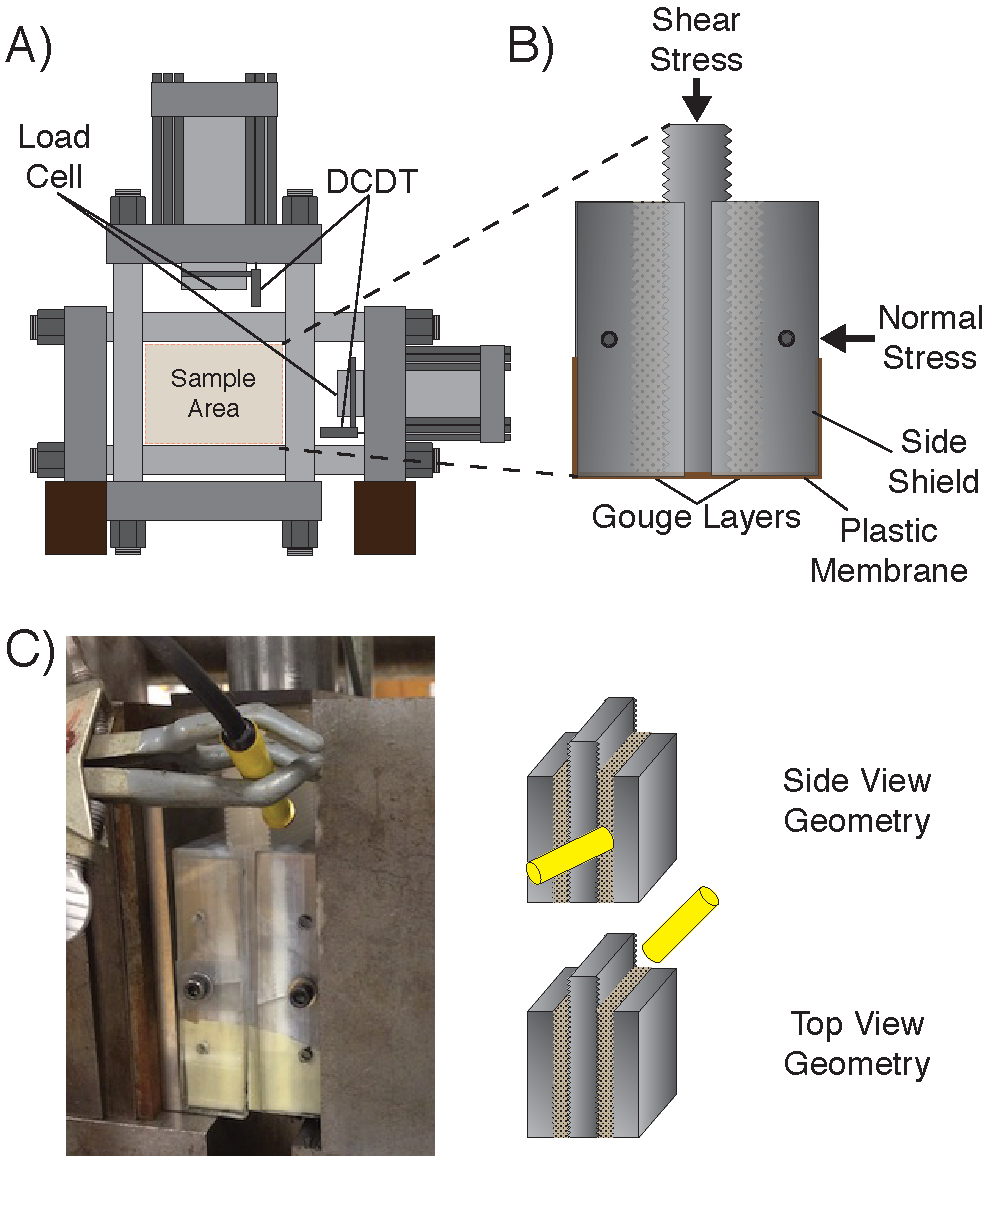
\includegraphics[width=30pc]{chap_electrical/biax_setup.pdf}
\caption{Experimental setup. A) The biaxial hydraulic press: sample assemblies are supported by steel blocks in the sample area. B) Double direct shear geometry consists of two layers of gouge confined between three forcing blocks.  Side shields and a plastic membrane are used to contain gouge material as the sample is sheared. C) Placement of the electrostatic voltmeter (yellow cylinder) in the side and top view positions.  A window was cut into the side shield for the side view geometry. }
\label{biax_setup}
\end{figure}

%% ---------------------------------- %%
%  Beads SEM Figure
%% ---------------------------------- %%
\begin{figure}
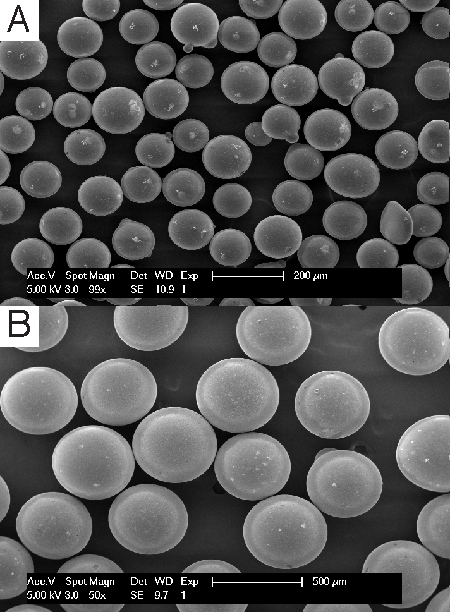
\includegraphics[width=30pc]{chap_electrical/sem_initial.pdf}
\caption{Scanning electron microscope micrographs of the starting glass beads for all experiments.  A) 100-150 $\mu m$ B) 420-500 $\mu m$}
\label{starting_SEM}
\end{figure}

%% ---------------------------------- %%
%  stick-slip Humidity
%% ---------------------------------- %%
\begin{figure}
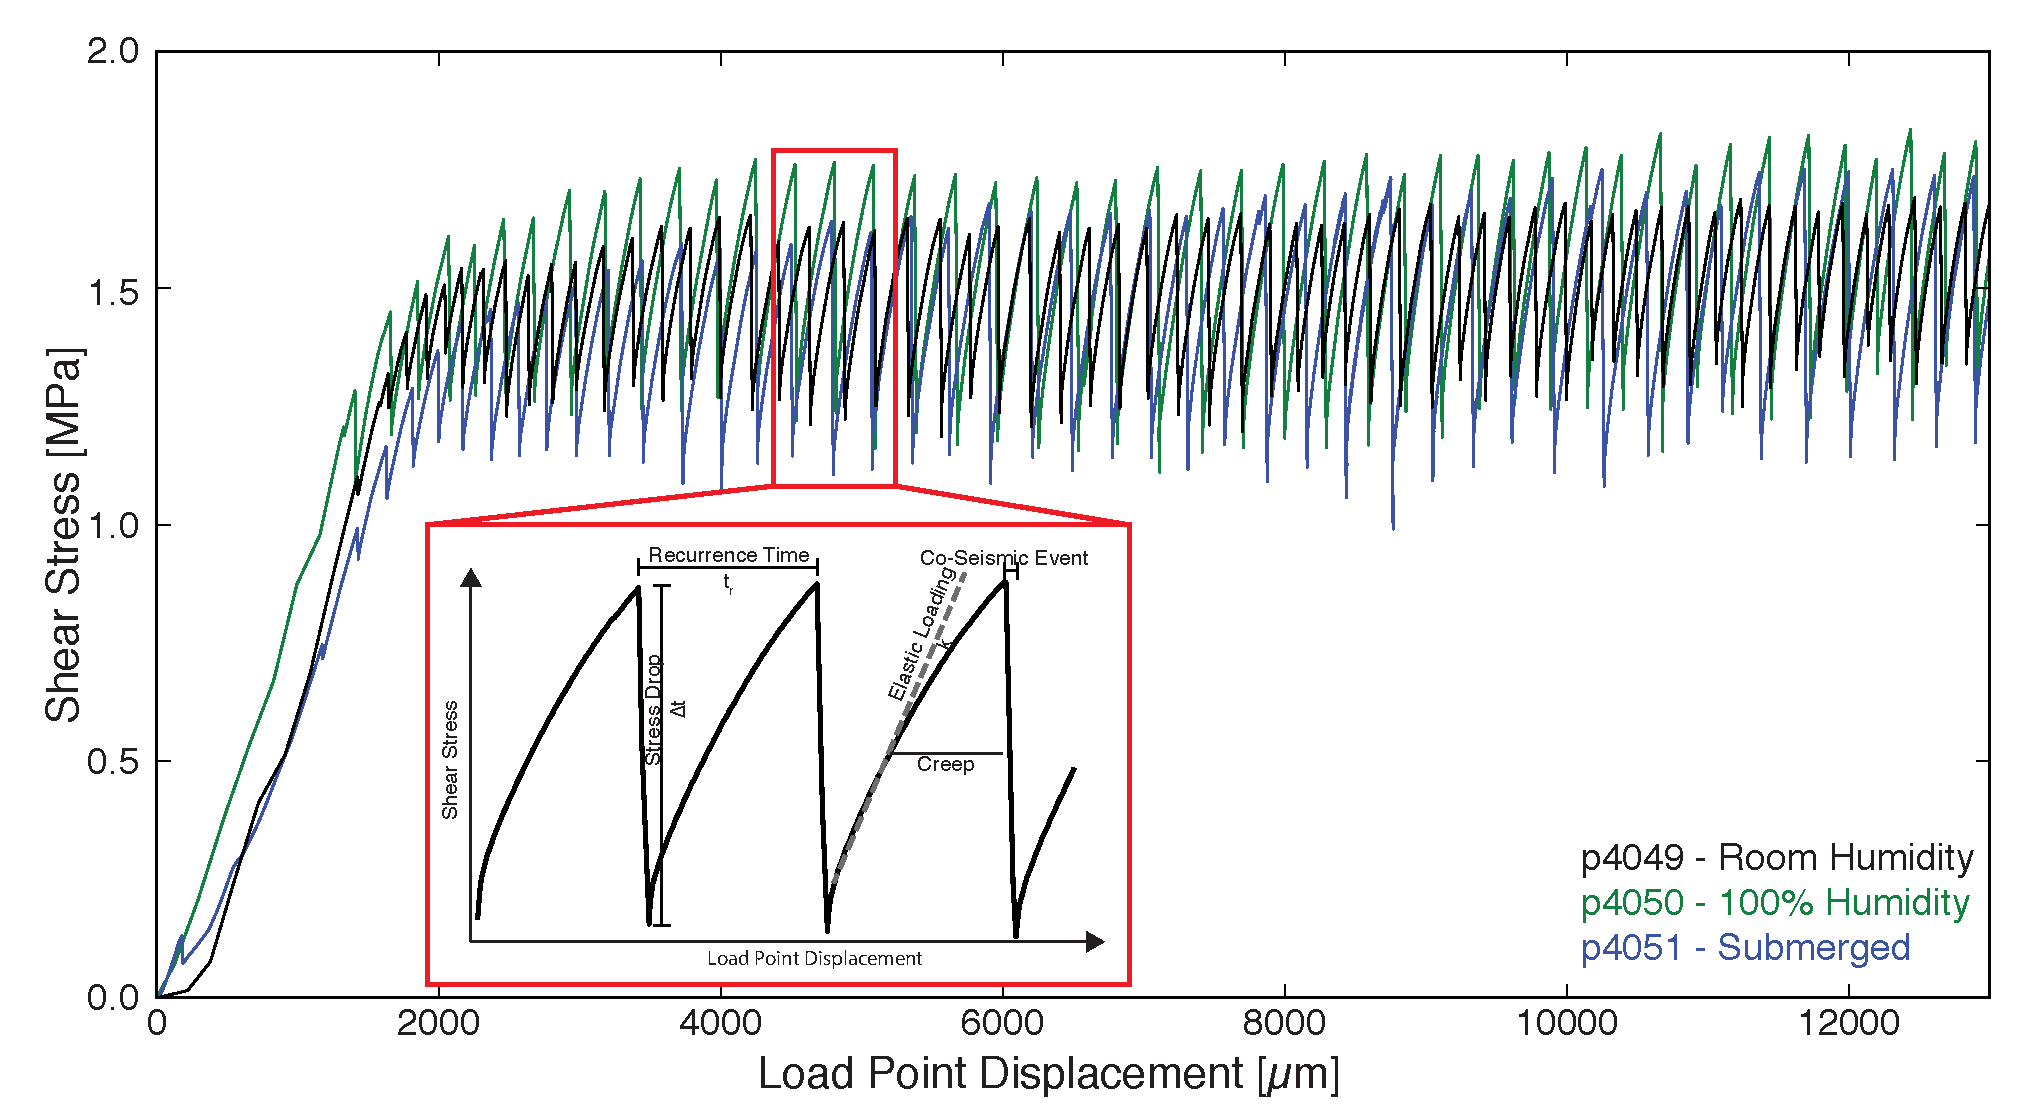
\includegraphics[width=40pc]{chap_electrical/ss_humidity.pdf}
\caption{Experiments performed on glass beads (100-150$\mu m$ diameter) under ambient humidity, 100\% humidity, and submerged conditions exhibit similar mechanical behavior.  Increased stress drops are observed with increased humidity and in the submerged case.  Inset: Anatomy of a stick-slip event.  The recurrence time is the time between peaks in shear stress.  Initially the shear stress increases linear-elastically.  Deviation from line-elastic behavior marks the onset of elasto-plastic deformation and pre-seismic slip.  When the ultimate strength of the layer is reached shear stress drops rapidly and the cycle begins again.}
\label{ss_humidity}
\end{figure}

%% ---------------------------------- %%
%  stick-slip Props
%% ---------------------------------- %%
\begin{figure}
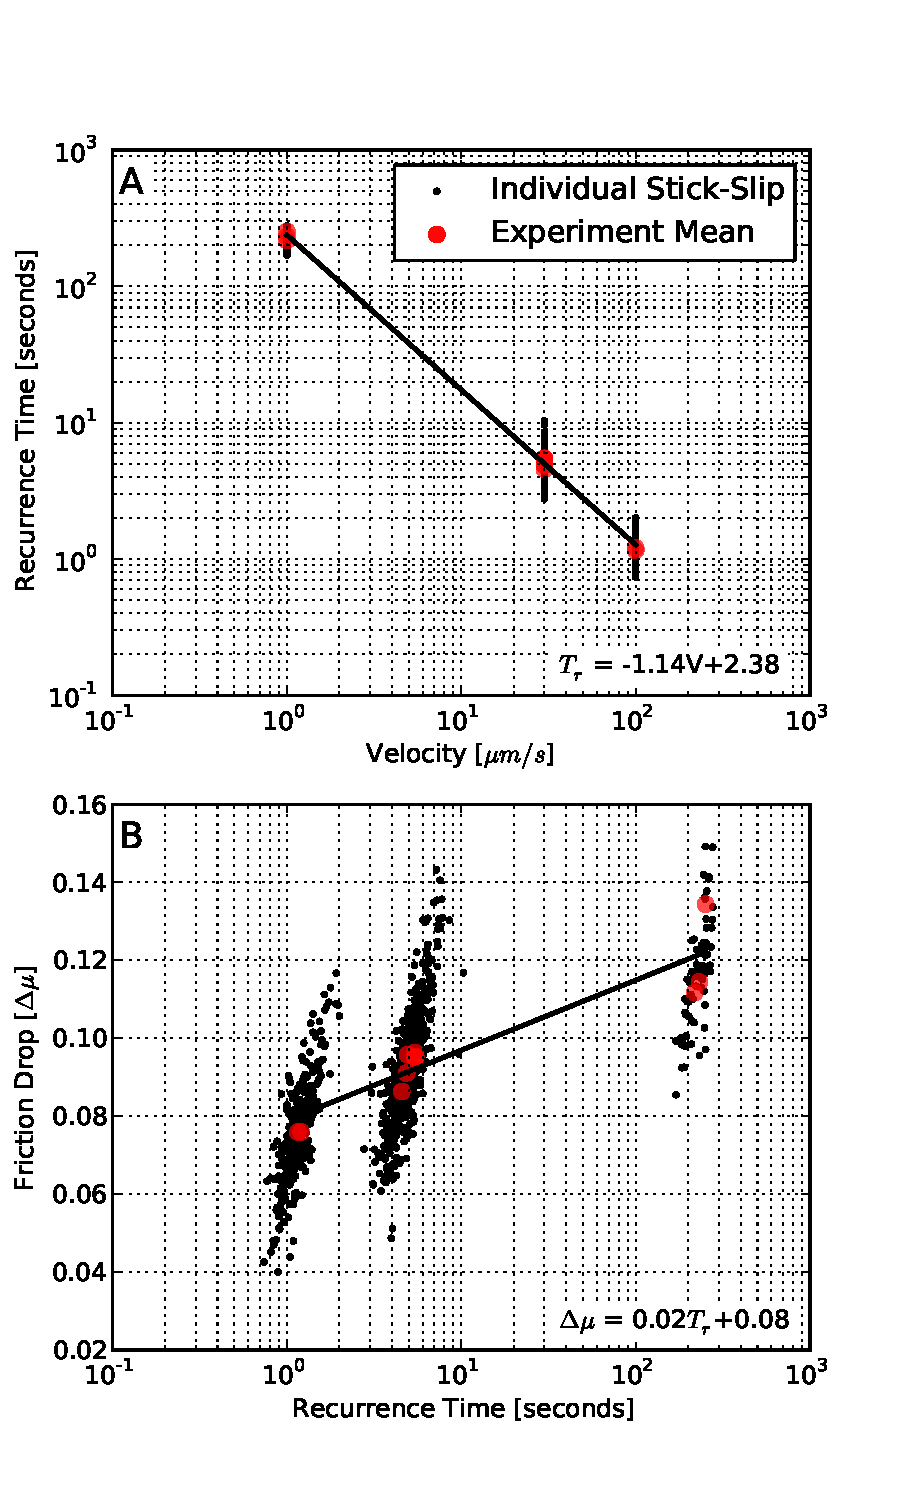
\includegraphics[width=25pc]{chap_electrical/ss_props.pdf}
\caption{A) Samples exhibit a log-log linear relation between recurrence time and velocity.  Faster loading rates result in shorter recurrence times. B) Friction drop increases with the recurrence time as there is more time for the layer to heal before the next stick-slip event.}
\label{ss_props}
\end{figure}

%% ---------------------------------- %%
%  Electrical Runplot
%% ---------------------------------- %%
\begin{figure}
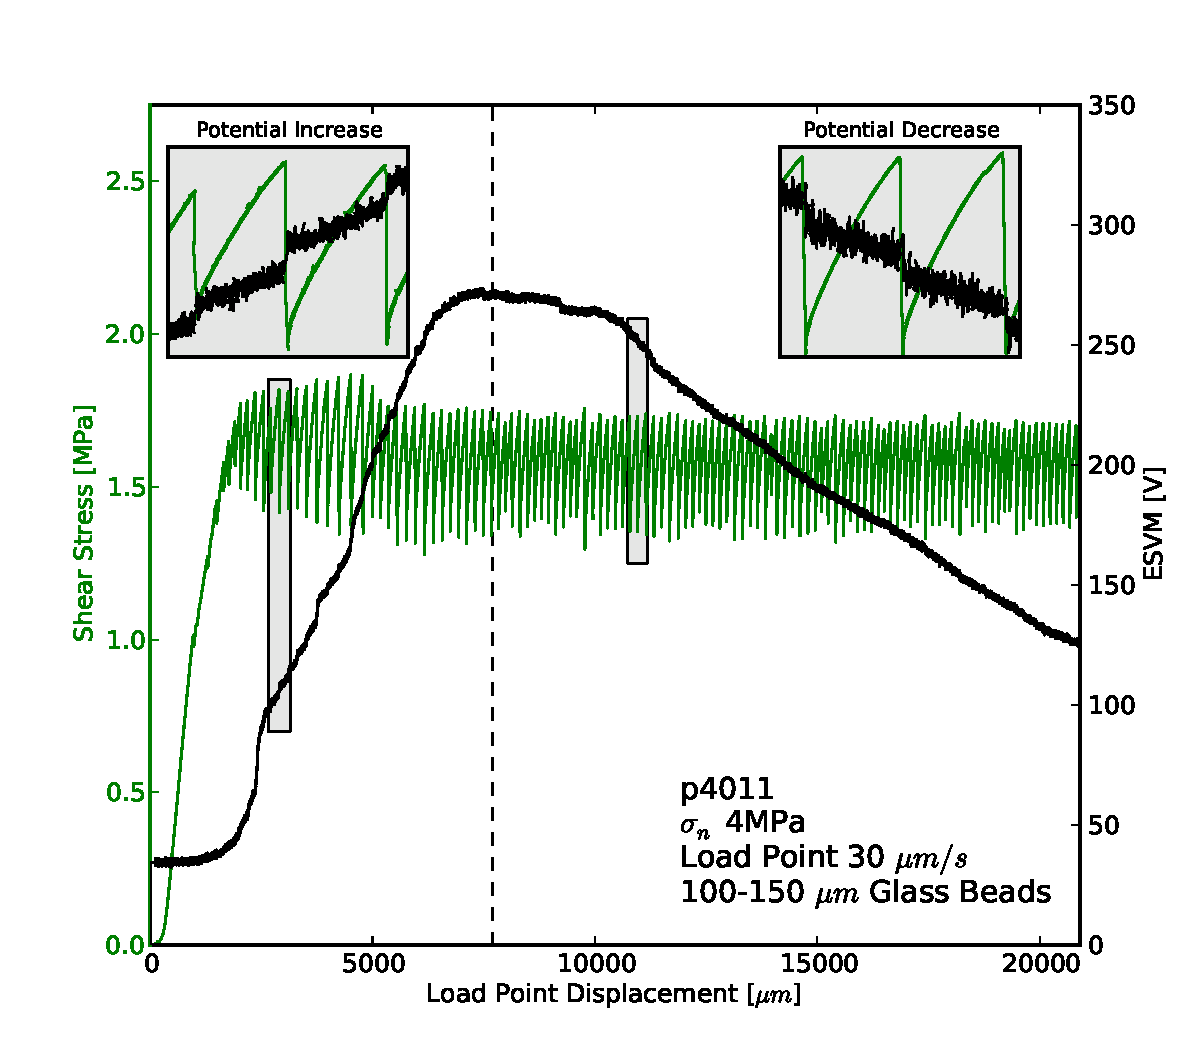
\includegraphics[width=40pc]{chap_electrical/elec_runplot.pdf}
\caption{During shearing two trends are observed: 1) A long-term charging/discharging trend in the electrical potential and 2) Potential change related to individual stick-slip events. The entire system initially charges, approximately until mechanical steady-state is reached. During this phase co-seismic potential changes are dominantly positive (top left inset).  After attainment of mechanical steady-state, the system begins to maintain or discharge potential.  During this phase the co-seismic potential changes are dominantly negative (top right inset).}
\label{electrical_runplot}
\end{figure}

%% ---------------------------------- %%
%  Electrical Zooms
%% ---------------------------------- %%
\begin{figure}
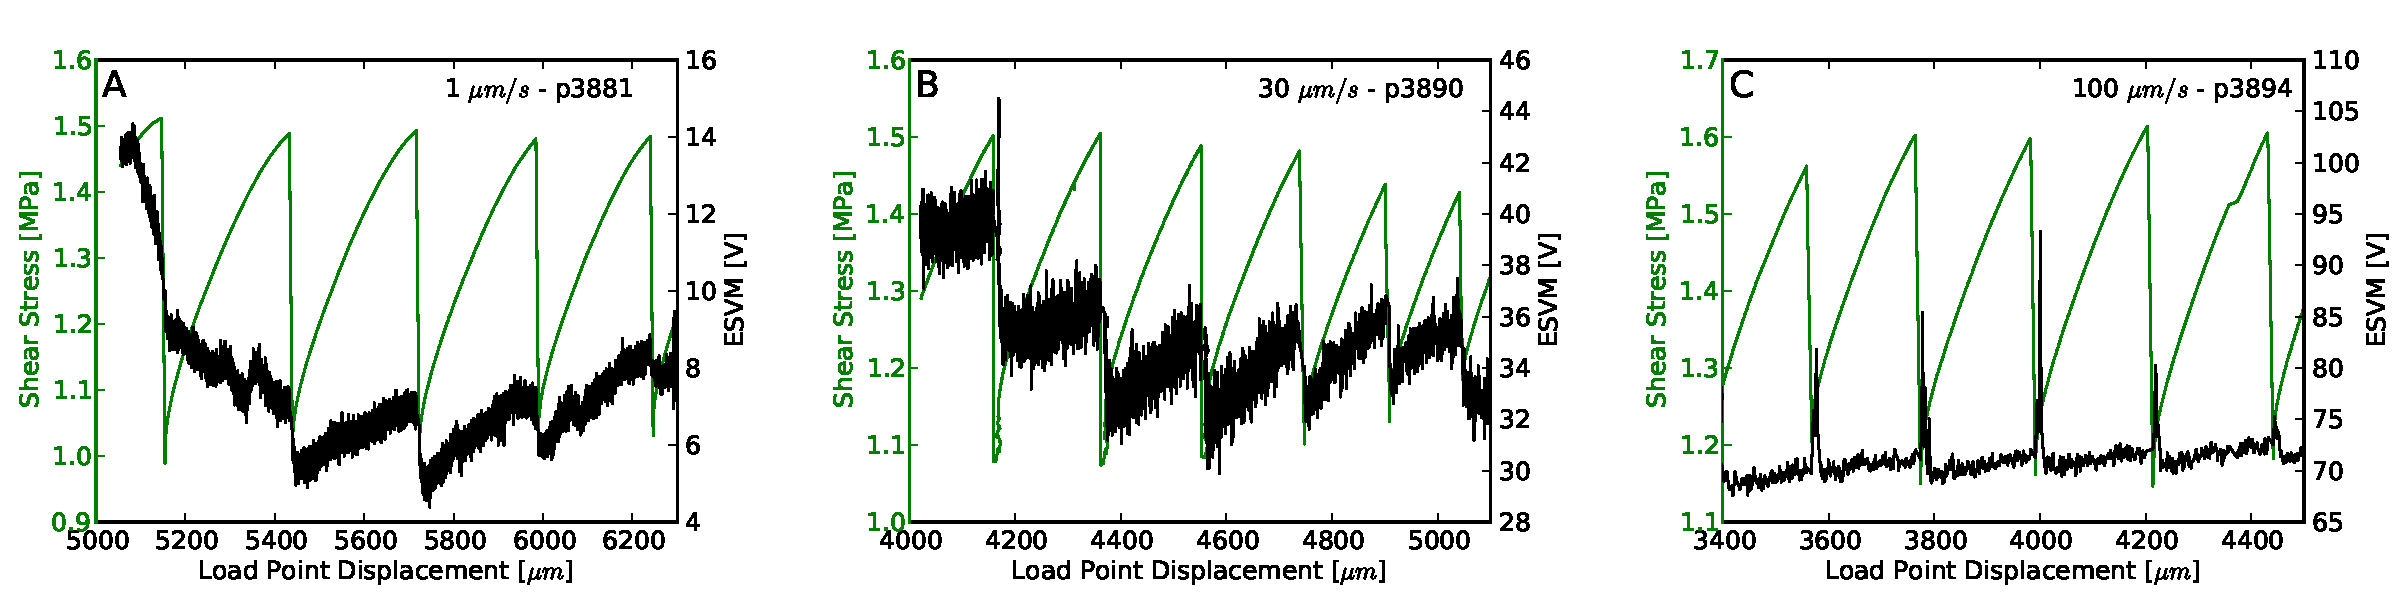
\includegraphics[width=45pc]{chap_electrical/elec_zooms.pdf}
\caption{Stick-slip events and associated ESVM measurements for three-different load point velocities of 1, 30, and 100 $\mu m/s$.  A) At slow loading velocities the electrical signal clearly mirrors the stress curve in most cases  B) For intermediate velocities, the relation is still present. C) At high velocities, the electrical signal is a sharp pulse an order of magnitude higher than those observed at low velocities, and we observe small inter-seismic charging.}
\label{electrical_zooms}
\end{figure}

%% ---------------------------------- %%
%  Voltage Change vs. Velocity log log
%% ---------------------------------- %%
\begin{figure}
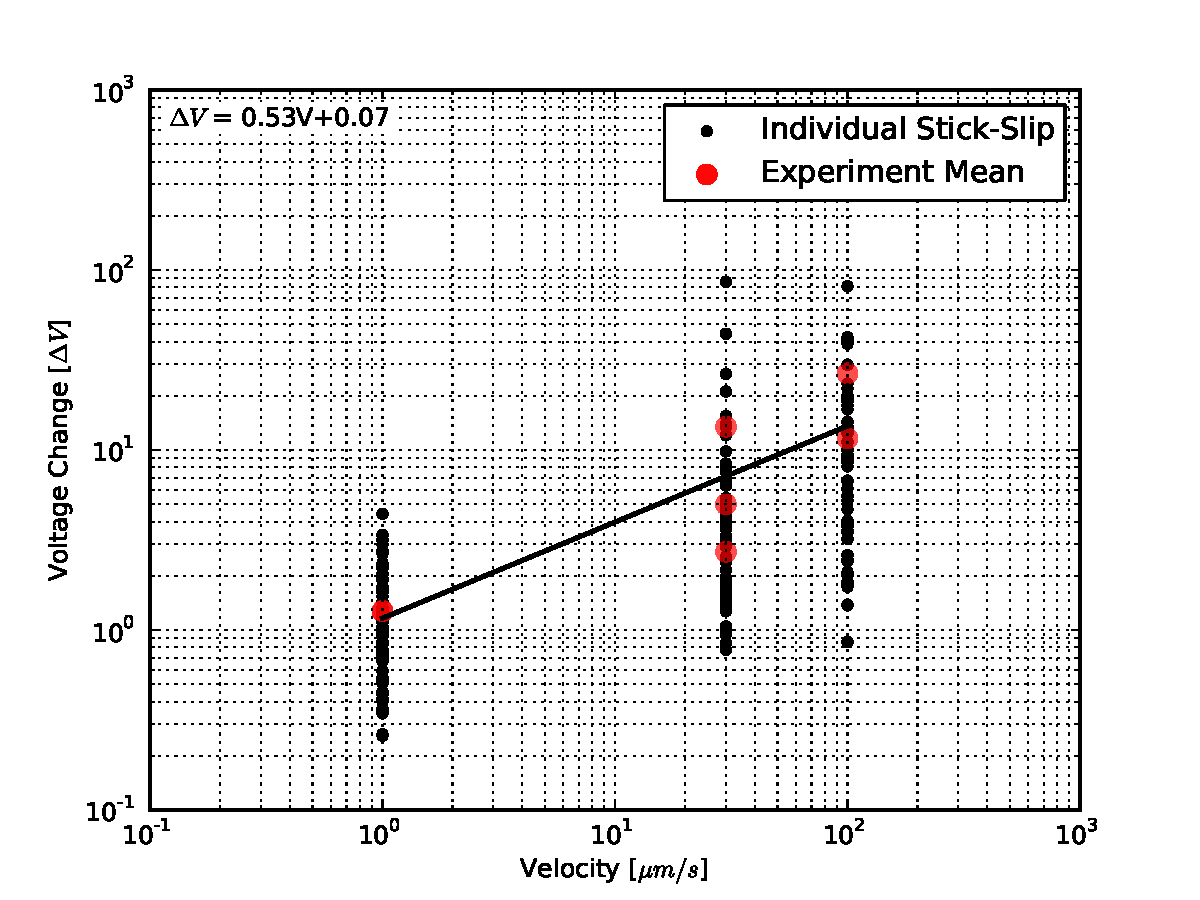
\includegraphics[width=30pc]{chap_electrical/vchange_velocity.pdf}
\caption{Each order of magnitude driving velocity change produces a $\sim$5x increase in the electrical signal observed.  All experiments shown are with the side-view sensor geometry.}
\label{voltage_velocity}
\end{figure}

%% ---------------------------------- %%
%  Model Cartoon
%% ---------------------------------- %%
\begin{figure}
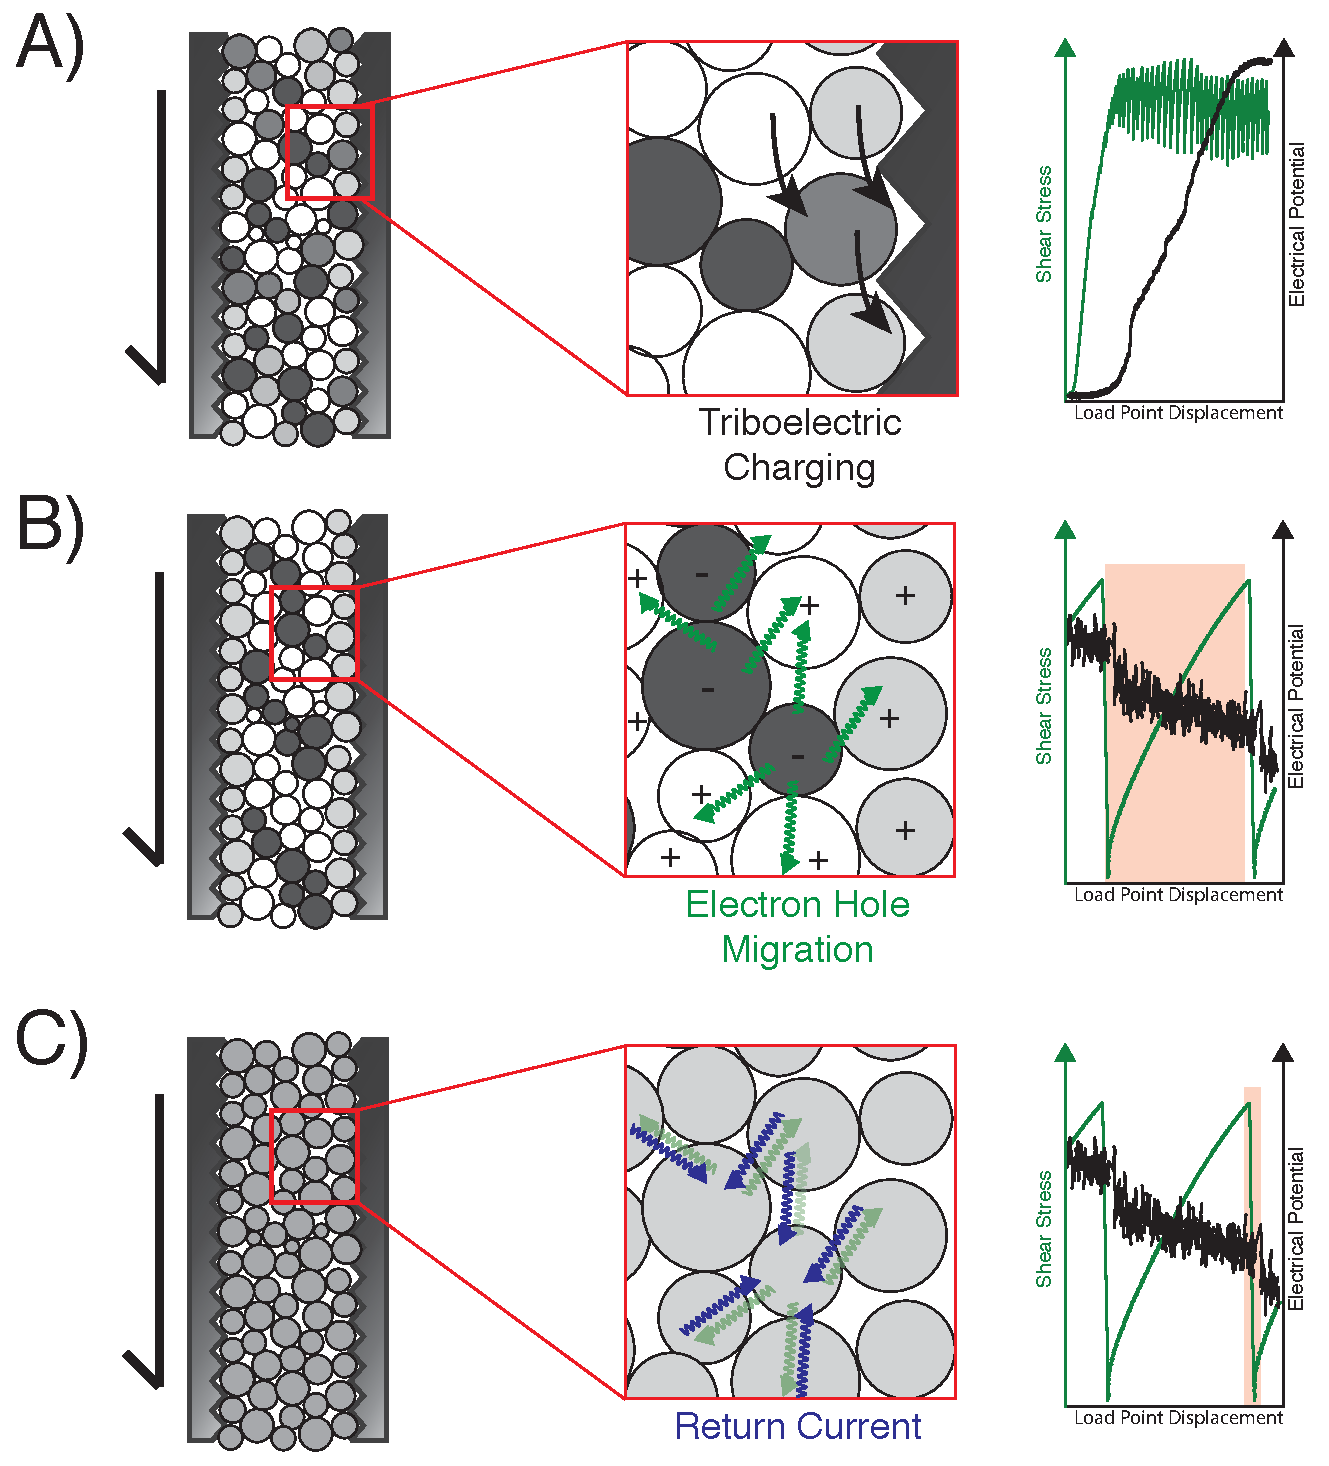
\includegraphics[width=30pc]{chap_electrical/model_cartoon.pdf}
\caption{A schematic representation of the stages of electrical behavior during an experiment:  A) During the initial run-in there is massive grain rearrangement as force chain networks begin to form.  This sliding motion tribo-electrically charges the system.  B) After the force chain network forms there is minimal grain-boundary sliding.  Shear loads are supported in the granular layer by highly stressed force chains (dark colors).  Electron holes migrate away from highly stressed beads into the matrix creating an electrical potential gradient.  C) When the layer fails and all grains are at roughly the same low stress, a return current redistributes the electrical gradient and the cycle begins again.}
\label{model_cartoon}
\end{figure}

%% ---------------------------------- %%
%  Appendix A - ESVM Calibration
%% ---------------------------------- %%
\begin{figure}
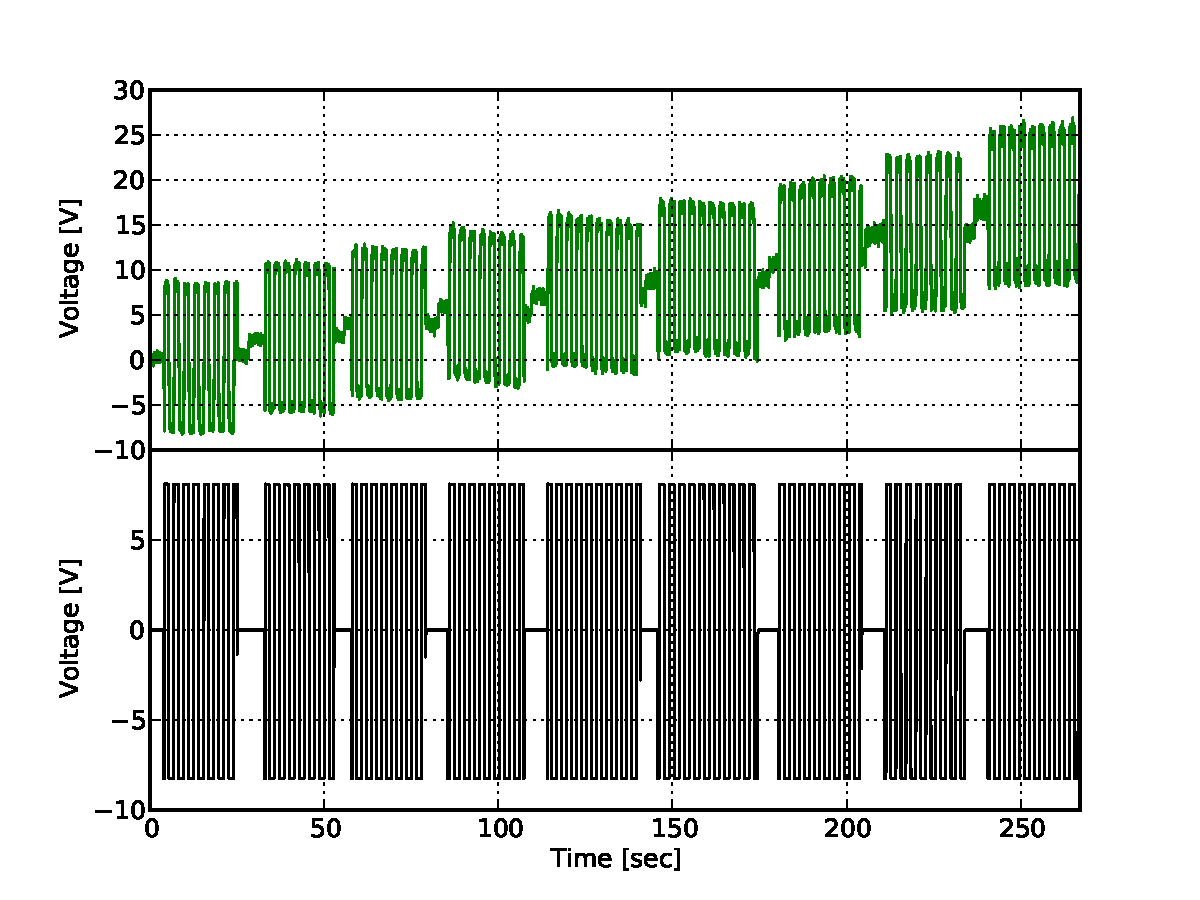
\includegraphics[width=30pc]{chap_electrical/ESVM_Calibration.pdf}
\caption{Calibration of the ESVM from a function generator source (bottom panel).  A series of steps through the ESVM `response' setting from 1-9 shows that the input square wave applied to the aluminium surface under test is well-recorded on each setting (top panel).  The upward trend in ESVM data is a product of a DC offset that occurs each time the response setting is changed on the instrument.}
\label{esvm_calibration}
\end{figure}

%% ---------------------------------- %%
%  Appendix A - ESVM response
%% ---------------------------------- %%
\begin{figure}
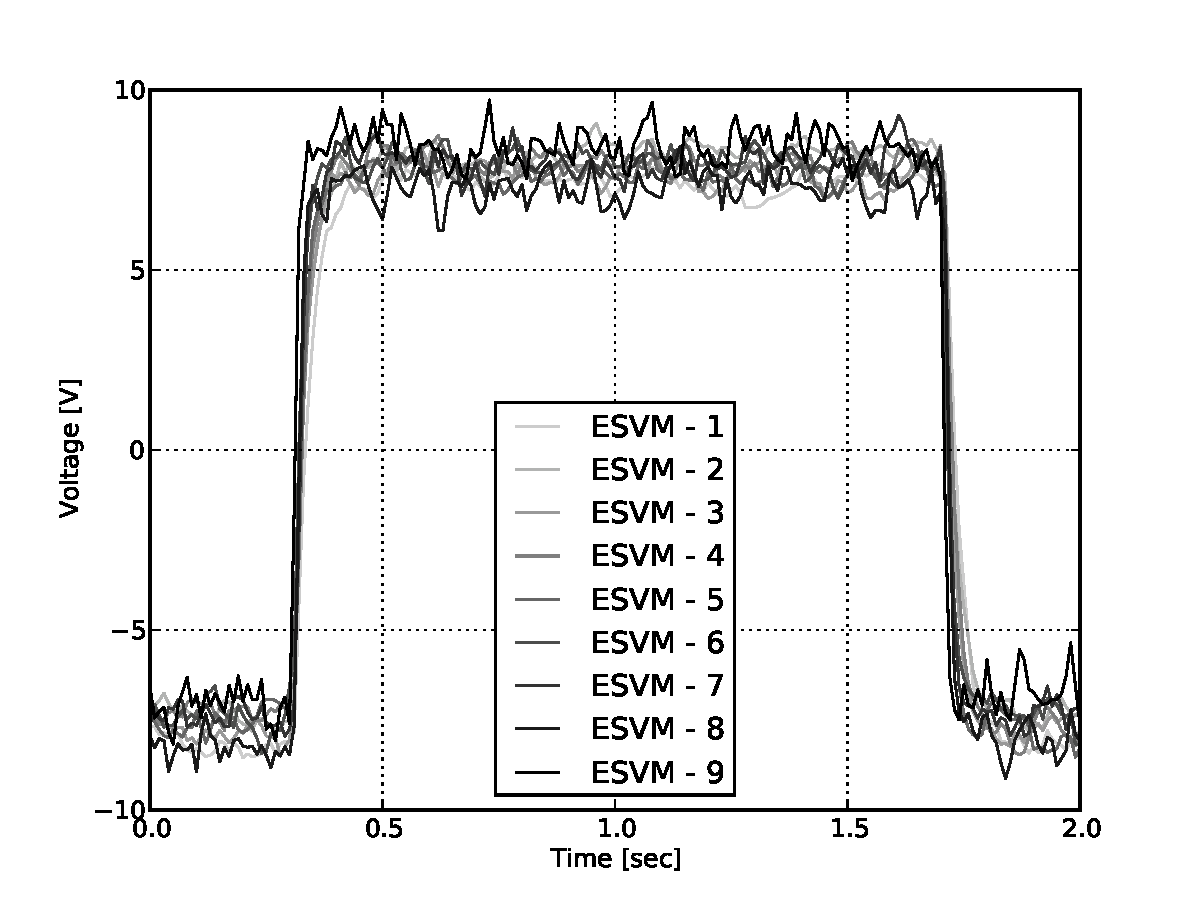
\includegraphics[width=30pc]{chap_electrical/ESVM_Calibration_Pulse.pdf}
\caption{A detailed comparison of a single waveform shows that at lower response settings (lighter colors) the waveform is smoothed slightly, with the nearly instantaneous voltage change distributed over up to 0.1 seconds on both the rise and fall.  At higher resolutions (darker colors) the sharp transition is clearly seen, but at the price of a higher noise level during the flat hold states.}
\label{esvm_response}
\end{figure}

%% ---------------------------------- %%
%  Appendix A - ESVM response timing
%% ---------------------------------- %%
\begin{figure}
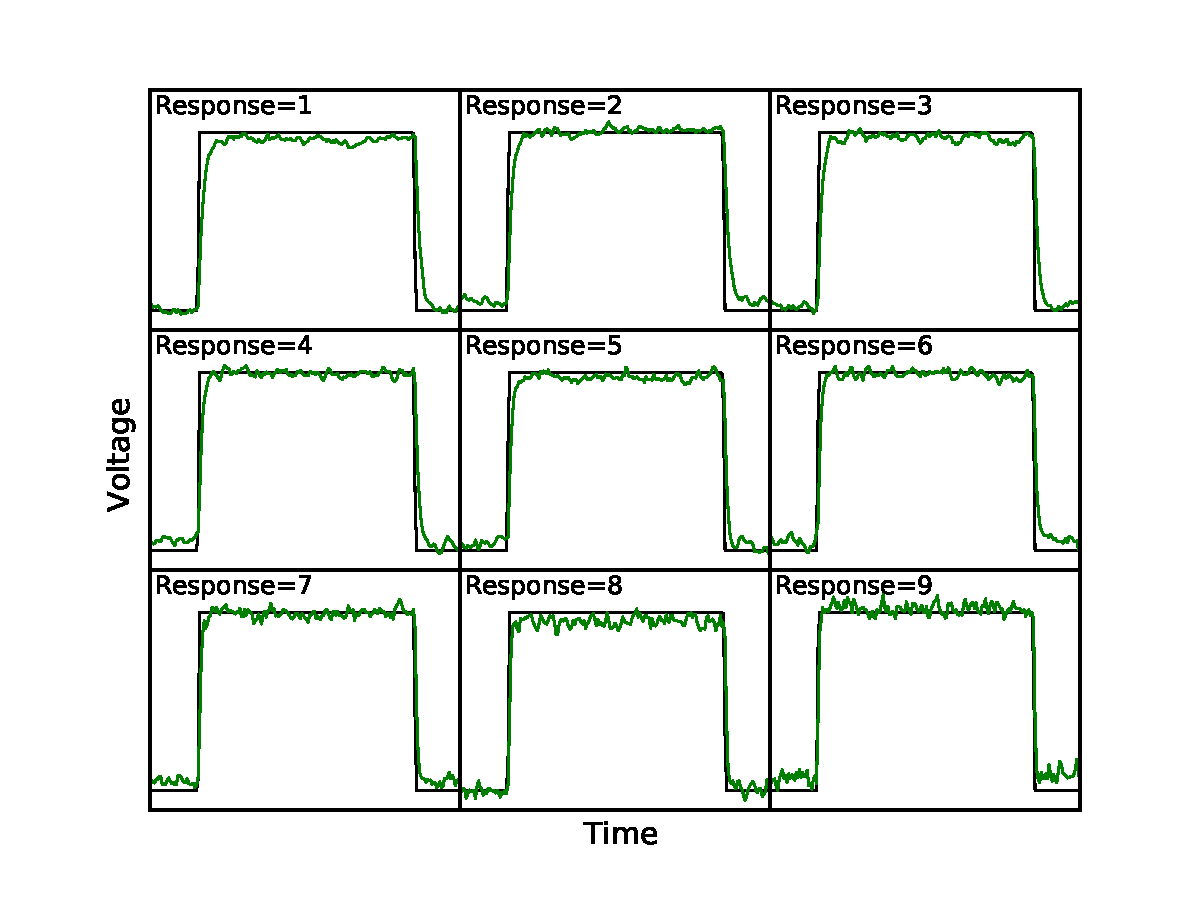
\includegraphics[width=30pc]{chap_electrical/ESVM_Allchan_timing.pdf}
\caption{At all response settings the beginning of ESVM signal change corresponds well in the time domain with the leading and falling edge of the input signal.  Smoothing due to longer integration times is observed at low response settings.}
\label{esvm_timing}
\end{figure}

%% ---------------------------------- %%
%  Table of Experiments
%% ---------------------------------- %%
\begin{table}
\caption{List of Experiments}
\centering
\begin{tabular}{c c c c c c}
\hline
 Experiment & $V_{lp}$, $\mu m/s$ & Bead Size, $\mu m$ & Temperature, $C^\circ$& Humidity, \%& Comment \\
\hline
p3853 & 30   & 420-500 & 23.3 & 41.2 & Large Beads\\
p3878 & 30   & 100-150 & 23.8 & 23.8 & Side View\\
p3879 & 30   & 420-500 & 24.7 & 20.2 & Large Beads\\
p3880 & 30   & 420-500 & 25.7 & 20.7 & Large Beads\\
p3881 & 30   & 100-150 & 26.9 & 20.7 & Side View\\
p3882 & 30   & 100-150 & 26.0 & 14.0 & Side View\\
p3887 & 30   & 100-150 & 22.7 & 22.5 & Side View\\
p3889 & 1     & 100-150 & 23.4 & 24.8 & Side View\\
p3890 & 100 & 100-150 & 24.1 & 33.8 & Side View\\
p3893 & 100 & 100-150 & 21.9 & 19.9 & Side View\\
p3894 & 1     & 100-150 & 22.7 & 19.8 & Side View\\
p4010 & 30   & 100-150 & 23.9 & 23.0 & Top View - Isolated Ground\\
p4011 & 30   & 100-150 & 24.2 & 23.7 & Top View\\
p4012 & 30   & 100-150 & 24.5 & 22.0 & Top View\\
p4013 & 1     & 100-150 & 24.3 & 22.3 & Top View\\
p4014 & 30   & 100-150 & 23.0 & 100  & Saturated\\
p4015 & 30   & 100-150 & 23.3 & N/A  & Submerged\\
p4049 & 30   & 100-150 & 23.9 & 27.0 & Control Test \\
p4050 & 30   & 100-150 & 23.8 & 100  & Saturated \\
p4051 & 30   & 100-150 & 23.9 & N/A  & Submerged \\
p4052 & 30   & 100-150 & 23.8 & 100  & Saturated \\
\hline
\label{exp_list}
\end{tabular}
\end{table}


%% ---------------------------------- %%
%  Table of Bead Composition
%% ---------------------------------- %%
\begin{table}
\caption{Composition of glass beads.}
\centering
\begin{tabular}{c c}
\hline
Compound & Composition,\%\\
\hline
SiO$_2$ & 65-75\% \\
Al$_2$O$_3$ & 0-5\%\\
CaO & 6-15\% \\
MgO & 1-5\%\\
Na$_2$O & 10-20\%\\
Fe$_2$O$_3$ & \textless 0.8\%\\
\hline
\label{bead_composition}
\end{tabular}
\end{table}